\subsection{Nos machines}
Dans le but d'étudier différents problèmes liés à la programmation par tâche, nous avons sélectionné deux machines avec des architectures différentes.


\subsubsection{Rostand}
Rostand est une grappe de serveurs appartenant à la compagnie Total S.A..
%
Elle est composée de 640 noeuds de calcul interconnectés avec un réseau Infiniband.
%
Chaque noeud est lui-même composé de 2 bancs NUMA avec un processeur Intel Xeon X5660 et 24~Go de mémoire par banc NUMA (Fig.~\ref{fig:rostand}).
%
Les processeurs ont 6 coeurs, soit un total de 12 coeurs par noeud de calcul et 7680 coeurs pour l'ensemble de la grappe.


%   (-_-)   %
\begin{figure}[!h]
        \centering
        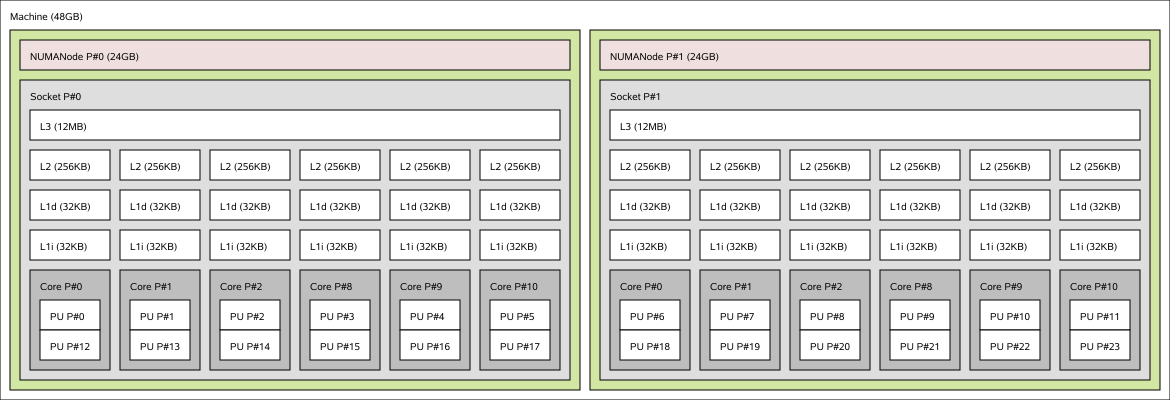
\includegraphics[width=\textwidth]{rostand_lstopo}
        \caption{Topologie d'un noeud de calcul de Rostand. Le schéma a été obtenu avec le logiciel hwloc.}
        \label{fig:rostand}
\end{figure}

Avec cette machine, nous allons pouvoir tester deux paradigmes de programmation parallèle.
%
Dans un premier temps nous utiliserons du parallélisme intra-noeud puis nous verrons le parallélisme inter-noeud.


La matrice des distances (Fig.~\ref{fig:rostand_distance}) nous indique la distance entre deux bancs NUMA donnée par le constructeur de la machine.
%
Cette distance est adimensionnée, la distance entre un banc NUMA et lui-même est égale à 10, les autres distances sont mises à l'échelle par rapport à 10 comme spécifié dans la norme ACPI.
%
Ces distances sont obtenues avec la commande {\em ``numactl --hardware''} sous Linux.
%
\'Etant donné que cette valeur ne peut servir qu'à connaître la topologie des bancs NUMA, nous avons décidé de mesurer la latence mémoire entre chaque banc.
%
Pour cela, nous avons utilisé l'outil {\em lmbench} couplé à {\em numactl} pour définir les bancs NUMA à utiliser.
%
Nous savons donc qu'un accès à un banc NUMA distant a un temps de latence 57~\% plus grand qu'un accès au banc NUMA local.


%   (-_-)   %
\begin{figure}[!h]
        \centering
        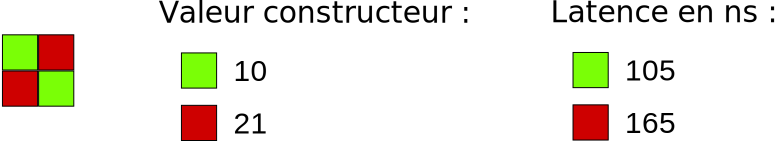
\includegraphics[width=0.5\textwidth]{rostand_distance}
        \caption{Matrice des distances entre chaque banc NUMA de Rostand.}
        \label{fig:rostand_distance}
\end{figure}

\subsubsection{Manumanu}
Manumanu est une machine Altix UV100, cet ordinateur est composé de 20 bancs NUMA.
%
Chaque banc NUMA est composé d'un processeur Intel Xeon E7-8837 ainsi que de 32~Go de mémoire.
%
Les processeurs ont chacun 8 coeurs de calcul, pour un total de 160 coeurs et 640~Go de mémoire partagée.
%
Cette machine est vraiment intéressante pour évaluer les effets NUMA.

%   (-_-)   %
\begin{figure}[!h]
     \begin{center}
        \subfigure[Matrice des distances entre chaque banc NUMA.]{%
          \label{fig:manumanu_distances}
          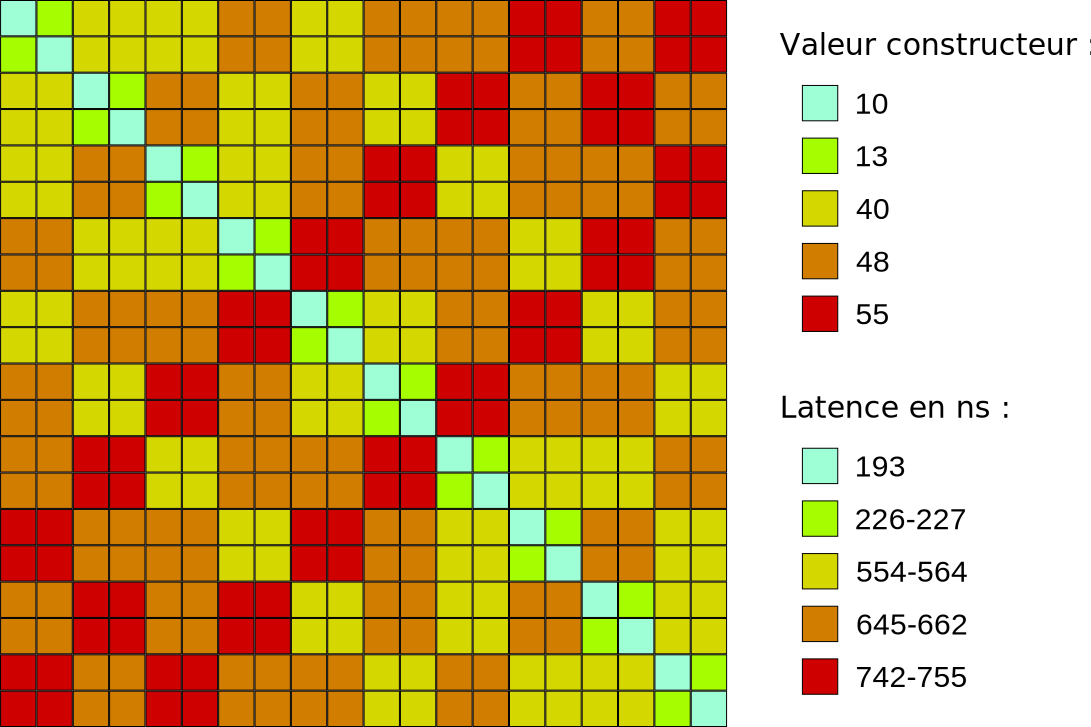
\includegraphics[width=0.59\textwidth]{manumanu_distance}
        }%
        \subfigure[Topologie déduite de la matrice des distances. Chaque noeud représente un groupe de deux bancs NUMA.]{%
          \label{fig:manumanu_topo}
          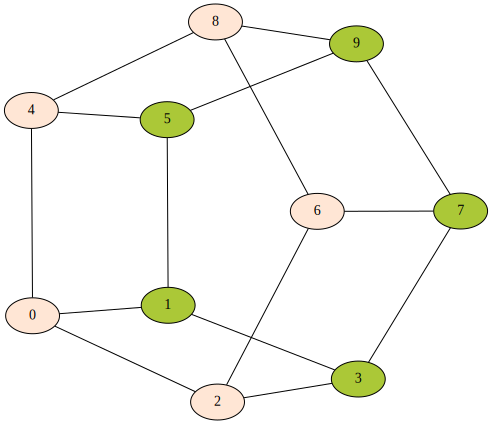
\includegraphics[width=0.39\textwidth]{manumanu_topologie}
        }%
    \end{center}
    \caption{Architecture de Manumanu.}
    \label{fig:manumanu}
\end{figure}

\`{A} partir de la matrice des distances (Fig.~\ref{fig:manumanu_distances}), nous pouvons déduire la topologie de la machine.
%
Les bancs NUMA sont regroupés deux par deux et chaque groupe est connecté à trois autres groupes.
%
Ce regroupement permet de limiter la distance maximal entre deux banc NUMA, il y aura au maximum 3 sauts.
%
Les temps de latence entre deux bancs NUMA d'un même groupe n'est supérieur que de 17\% par rapport à un accès local.
%
Par contre, les temps de latence entre deux groupes sont entre 3 et 4 fois plus long qu'un temps de latence local.
